\documentclass[]{interact}

%\usepackage[caption=false]{subfig}% Support for small, `sub' figures and tables
%\usepackage[nolists,tablesfirst]{endfloat}% To `separate' figures and tables from text if required
%\usepackage[doublespacing]{setspace}% To produce a `double spaced' document if required
%\setlength\parindent{24pt}% To increase paragraph indentation when line spacing is doubled
%\setlength\bibindent{2em}% To increase hanging indent in bibliography when line spacing is doubled

\usepackage[numbers,sort&compress]{natbib}% Citation support using natbib.sty
\bibpunct[, ]{[}{]}{,}{n}{,}{,}% Citation support using natbib.sty
\renewcommand\bibfont{\fontsize{10}{12}\selectfont}% Bibliography support using natbib.sty

\usepackage{amsmath,amssymb}
\usepackage{stmaryrd}  % \llbracket, \rrbracket

\usepackage[T1]{fontenc}
\usepackage{caption,subcaption}

\usepackage{pgfplots}
\usetikzlibrary{arrows}
\pgfplotsset{compat=1.16}

\usepackage{algorithm}
\usepackage[noend]{algpseudocode}

\usepackage{minted}

\usepackage[hidelinks]{hyperref}

\theoremstyle{plain}% Theorem-like structures provided by amsthm.sty
\newtheorem{theorem}{Theorem}[section]
\newtheorem{lemma}[theorem]{Lemma}

\newtheorem{corollary}[theorem]{Corollary}
\newtheorem{proposition}[theorem]{Proposition}

\theoremstyle{definition}
\newtheorem{definition}[theorem]{Definition}
\newtheorem{example}[theorem]{Example}

\theoremstyle{remark}
\newtheorem{remark}{Remark}
\newtheorem{notation}{Notation}

\newcommand{\RR}{\mathbb{R}}

\newcommand{\eps}{\epsilon}
\newcommand{\grad}{\nabla}
\newcommand{\Div}{\nabla\cdot}

\newcommand{\bn}{\mathbf{n}}
\newcommand{\bq}{\mathbf{q}}

\newcommand{\bX}{\mathbf{X}}

\newcommand{\cK}{\mathcal{K}}
\newcommand{\cT}{\mathcal{T}}
\newcommand{\cX}{\mathcal{X}}
\newcommand{\cY}{\mathcal{Y}}

\newcommand{\CG}{\text{CG}}
\newcommand{\DG}{\text{DG}}


\begin{document}

%\articletype{ARTICLE TEMPLATE}% Specify the article type or omit as appropriate

\title{Adaptive mesh refinement for obstacle problems}

\author{
\name{G.~Stefano Fochesatto\thanks{CONTACT G.~Stefano Fochesatto Email: gsfochesatto@alaska.edu} and Ed Bueler}
\affil{Dept.~of Mathematics and Statistics, University of Alaska Fairbanks, USA}
}

\maketitle

\begin{abstract}
Free-boundary problems posed as variational inequalities, including obstacle problems, appear in many scientific and engineering applications.  In the finite element solution of these problems, the geometrical error in locating the unknown free boundary often dominates the overall numerical error.  In this paper we propose, and implement using the Firedrake finite element library, parallel adaptive mesh refinement strategies which enhance mesh resolution around the free boundary.  These methods mark elements for refinement based on a computed solution.  We consider three methods: (i) an unstructured dilation operator which computes discrete adjacency to the computed free-boundary; (ii) a variable-coefficient diffusion method which thresholds a diffused indicator function for the computed active set; and (iii) a metric-based method which averages an anisotropic, Hessian-derived Riemannian metric with an isotropic metric computed from the same diffused indicator as in method (ii).  The addition of classical \emph{a posteriori} error estimators within the computed inactive sets is necessary to attain convergence.  These methods are evaluated by norm error and free-boundary localization error, versus mesh complexity and run-time.  Applications include classical Laplacian obstacle problems and a shallow ice flow problem for predicting glaciation of a land surface.
\end{abstract}

%\begin{keywords}
%FIXME
%\end{keywords}


\section{Introduction} \label{sec:intro}

The classical Laplacian obstacle problem \cite{KinderlehrerStampacchia1980} finds the equilibrium position (vertical displacement) $u$ of an elastic membrane over some domain $\Omega \subset \RR^d$.  The membrane, attached with displacement $g$ at the fixed boundary $\partial\Omega$ and subjected to an applied force $f$, is constrained to be above a given obstacle $\psi$.  The strong formulation of this problem is this complementarity problem over $\Omega$:
\begin{subequations} \label{eq:classical:ncp}
\begin{align}
  -\nabla^2 u - f \geq 0 \label{eq:classical:ncp:a} \\
  u - \psi \geq 0\\
  (-\nabla^2u - f)(u - \psi) = 0 \label{eq:classical:ncp:c}
\end{align}
\end{subequations}
From a solution to \eqref{eq:classical:ncp}, or rather from solving its weak form (given momentarily), we may identify the inactive and active sets,
\begin{equation}
  I_u = \{x \in \Omega \,:\, u(x) > \psi(x)\}, \quad A_u = \Omega \setminus I_u, \label{eq:classical:sets}
\end{equation}
and the free boundary
\begin{equation}
\Gamma_u = \Omega \cap \partial I_u. \label{eq:classical:freeboundary}
\end{equation}
Note that $u$ solves the Poisson equation $-\nabla^2u = f$ on $I_u$, the interior condition of the free-boundary problem.  Both Dirichlet ($u=\psi$) and Neumann ($\partial u/\partial n = \partial \psi/\partial n$) conditions apply along the unknown set $\Gamma_u$, but only Dirichlet conditions hold on $\partial\Omega$.

For the example shown in Figure \ref{fig:ball}, the obstacle $\psi$ is an upper hemisphere, the active set $A_u$ is a disc (white mesh), and the free boundary $\Gamma_u=\partial A_u$ is a circle.

\begin{figure}[H]
\centering
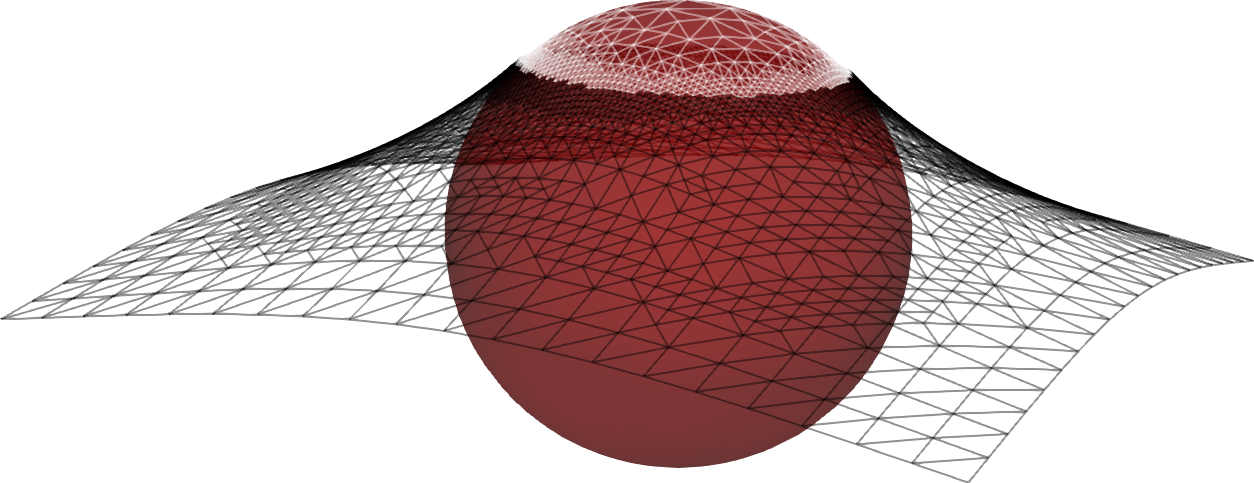
\includegraphics[width=0.8\textwidth]{static/obstacle.png}
\caption{Solution, as wireframe, to a problem with a (hemi)spherical obstacle.}
\label{fig:ball}
\end{figure}

Another physical interpretation of problem \eqref{eq:classical:ncp} is where $u$ models the pressure in a porous dam, which cannot go below zero ($\psi=0$); see examples in \cite{AinsworthOdenLee1993} and \cite{Bueler2021}.

As is well-known, problem \eqref{eq:classical:ncp} has a weak formulation which is a variational inequality (VI) over a Sobolev space.  Let $\cX=H^1(\Omega)$ \cite{ElmanSilvesterWathen2014} and suppose $\psi \in \cX \cap C(\bar\Omega)$.  (If it were a faithful visualization, Figure \ref{fig:ball} would show $\psi$ as an upper hemisphere extended continuously to $\partial\Omega$.)  Let $g:\partial \Omega\to \RR$ be continuous, with $g\ge\psi|_{\partial \Omega}$.  Let
\begin{equation} \label{eq:classical:admissible}
\cK = \{u \in \cX \,:\, u \ge \psi \text{ and } u|_{\partial \Omega} = g\}
\end{equation}
be the admissible subset, closed and convex in $\cX$.  For $f\in L^2(\Omega)$, the VI formulation of the obstacle problem \cite{KinderlehrerStampacchia1980} finds $u\in \cK$ so that
\begin{equation} \label{eq:classical:vi}
\int_\Omega \nabla u \cdot \nabla(v - u) \ge \int_\Omega f(v - u) \quad \text{ for all } v \in \cK.
\end{equation}

In Section \ref{sec:vifem} we will recall some of the theory of such VIs, and their finite element (FE) approximation.  However, we will generalize from elliptic bilinear forms like \eqref{eq:classical:vi} to coercive nonlinear operators over Banach spaces.  A conforming FE approximation $u_h$ of the VI solves the same weak form, but now over a finite-dimensional admissible set constructed on a mesh $\cT_h$.  Similarly to Cea's lemma for PDEs \cite{ElmanSilvesterWathen2014}, the norm errors $\|u-u_h\|$ can be bounded \emph{a priori} by extending the Falk \cite{Falk1974} technique to nonlinear operators.  In fact, Theorem \ref{thm:genfalk} will show how norm errors are controlled by the approximation properties of the FE space, but also subject to VI-specific concerns regarding admissibility and the construction of the FE obstacle.

Adaptive mesh refinement (AMR) uses \emph{a posteriori} information from the numerical solution over a given mesh to strategically add elements to the mesh to reduce the  numerical error.  However, for VI problems the geometrical error in locating the free-boundary $\Gamma_u$ on a mesh can, by itself, influence the global error $\|u-u_h\|$.  This fact, somewhat acknowledged in the FE literature for VIs \cite{Suttmeier2008}, is clearly seen in the following 1D example.

\begin{example} \label{example:oned} Suppose $\Omega = (-1,1)$, $\psi(x)=0.5 - x^2$, $f=0$, and $g=0$.  The exact solution $u$ of \eqref{eq:classical:vi} for this data is easily calculated.  Free boundaries are at $x_*=\pm(1-2^{-1/2})$ (Figure \ref{fig:parabola}).  For an FE approximation using piecewise-linear elements and a uniform mesh, let $\Delta_h$ be the minimum distance between a node and $x_*$.  Noting that $x_*$ are irrational, under uniform refinements $\Delta_h = O(h)$ is an irregular function of $h$.  Figure \ref{fig:parabola} (right) compares $H^1$ and $L^2$ norm errors to $\Delta_h$.  The erratic behavior of the norm errors closely follows the purely-geometrical free-boundary location error $\Delta_h$. \end{example}

\begin{figure}[ht]
\noindent \mbox{
\begin{minipage}[t]{0.45\textwidth}
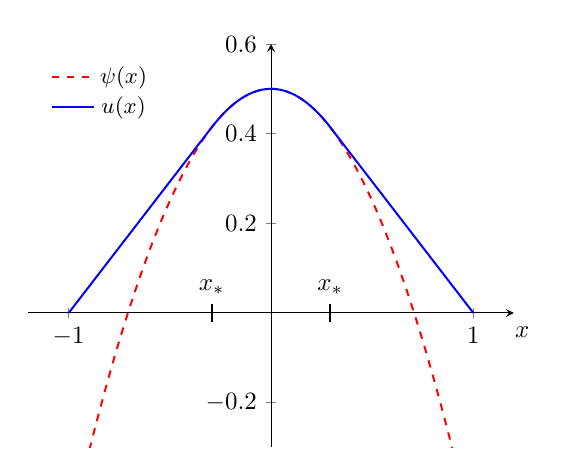
\begin{tikzpicture}[scale=0.9]
    \begin{axis}[
      axis lines = middle,
      xlabel = {$x$},
      xlabel style = {at={(1.05, 0.25)}},  % relative to whole figure box [0,1]x[0,1]
      domain = -1:1,
      samples = 100,
      xmin = -1.2,
      xmax = 1.2,
      ymin = -0.3,
      ymax = 0.6,
      xtick = {-1,1},
      legend pos = north west,
      legend style = {draw=none, font=\small}
    ]
      % Parameters
      \def\b{(2-sqrt(2))/2}
      \def\a{-\b}
      % Plot the obstacle function psi(x)
      \addplot[
        thick,
        red,
        dashed
      ] {0.5 - x^2};
      \addlegendentry{$\psi(x)$}
  
      % Plot u(x) in three pieces
      \addplot[
        thick,
        blue,
        domain=-1:\a
      ] {((.5 - \a*\a)/(\a + 1))*(x + 1)};
      \addplot[
        thick,
        blue,
        domain=\a:\b
      ] {0.5 - x^2};
      \addplot[
        thick,
        blue,
        domain=\b:1
      ] {-((.5 - \b*\b)/(1 - \b))*(x - 1)};
      \addlegendentry{$u(x)$}

      % indicate free boundary locations
      \addplot[black, thick, draw] coordinates {(\a,-0.02) (\a,0.02)} node[above] (A) {$x_*$};
      \addplot[black, thick, draw] coordinates {(\b,-0.02) (\b,0.02)} node[above] (B) {$x_*$};
    \end{axis}
  \end{tikzpicture}
  
\end{minipage}
\,
\begin{minipage}[t]{0.53\textwidth}
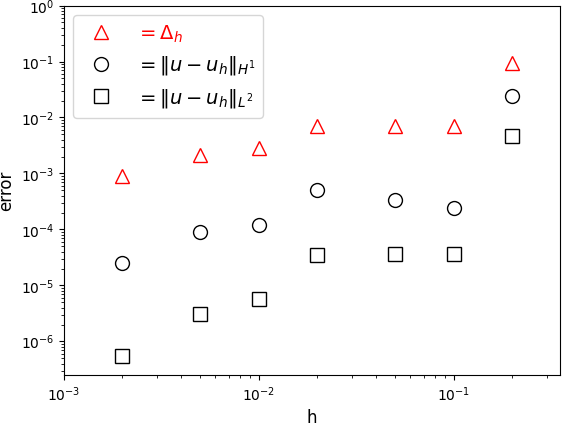
\includegraphics[width=\textwidth]{static/VIConvergence.png}
\end{minipage}
}
\caption{A one-dimensional obstacle problem (left), for which the geometrical free-boundary location error $\Delta_h$ predicts norm error $\|u-u_h\|$ behavior (right).}
\label{fig:parabola}
\end{figure}

A small modification of Example \ref{example:oned} illustrates another aspect of obstacle problems, namely that the sets $A_u,I_u,\Gamma_u$ are generally \emph{not} continuous functions of the data.

\begin{example} \label{example:notcontinuous} Suppose we change Example \ref{example:oned} by setting $g=-0.5$, so that $g=\psi$ on $\partial\Omega$.  For $\eps\in\RR$ we define a new source term $f_\eps(x)=2+\eps$.  An easy calculation shows that for $\eps\le 0$ the solution is $u_\eps=\psi$, thus $A_{u_\eps}=\Omega$ and $I_{u_\eps}=\emptyset$.  However, for $\eps>0$, so that $f_\eps$ represents sufficient upward force on the membrane to lift it off the obstacle, we find the solution satisfies $u_\eps(x)=\psi(x) + 0.5\, \eps\, (1-x^2) > \psi(x)$ for all $x\in\Omega$.  Thus $A_{u_\eps}=\emptyset$ and $I_{u_\eps}=\Omega$ for $\eps>0$, so these sets are discontinuous functions at $\eps=0$. \end{example}

By definition, the $\eps=0$ case of Example \ref{example:notcontinuous} is \emph{degenerate} \cite{KinderlehrerStampacchia1980}, that is, the unconstrained solution happens to match the obstacle.  This example shows that any predictable convergence results for FE approximations of the solution-dependent sets $A_u,I_u,\Gamma_u$ will depend upon nondegeneracy assumptions of some kind.

In fact, the effectiveness of different AMR strategies for VI problems depends upon the measure (area or volume) of the active and inactive sets.  This observation motivates the \emph{a posteriori} considerations in Section \ref{sec:aposteriori}.  For certain obstacle-type problems, specifically those with a ``blistering'' property, elements significantly interior to the active set may require no further computation or refinement.  For such problems, if a solution is desired at higher resolution within the active set where $u=\psi$ then this can be computed in post-processing by arbitrary interpolation of the obstacle.  That is, $\psi$ has already been provided in the data of the problem.

\begin{example} \label{example:activesets} Examples in Section \ref{sec:results} will measure convergence rates for three 2D classical obstacle problems.  Figure \ref{fig:activesizes} shows high-resolution active sets for these examples.  For the right-most case, with a large active set, we will see that most of the performance benefit of our preferred AMR techniques, relative to uniform refinement, comes from avoiding refinement in the active set.  This benefit also dominates performance gains in our glaciation application (Section \ref{sec:app}). \end{example}

\begin{figure}[ht]
\noindent \hspace{-1mm} \mbox{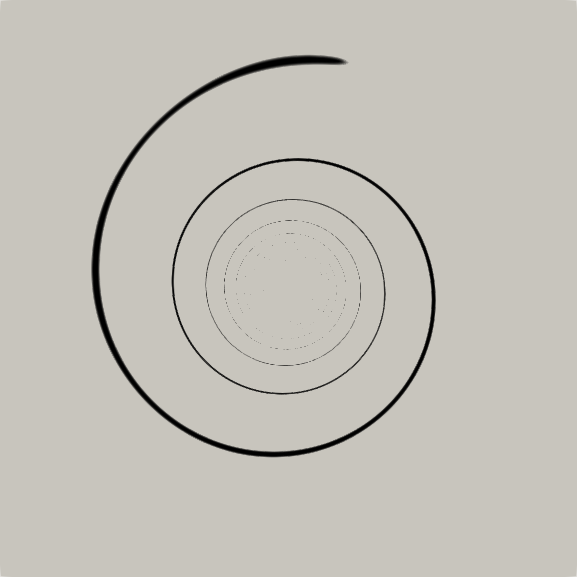
\includegraphics[width=0.32\textwidth]{static/spiral.png} \, 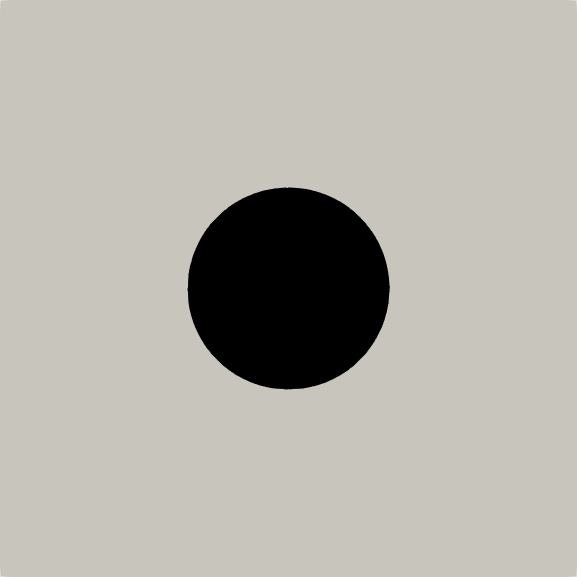
\includegraphics[width=0.32\textwidth]{static/sphere.png} \, 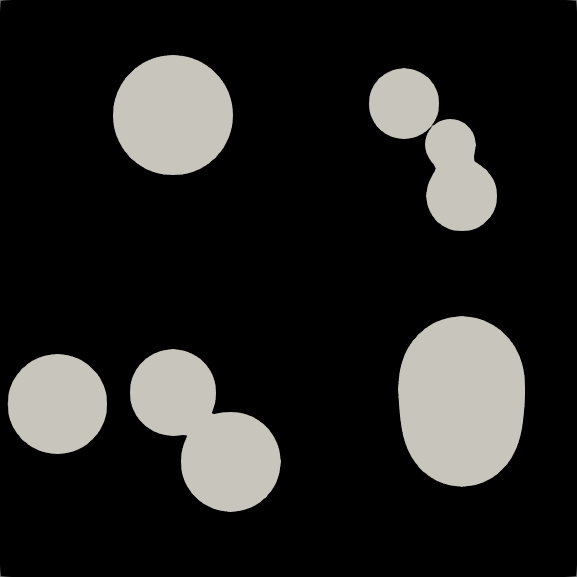
\includegraphics[width=0.32\textwidth]{static/blisters.png}}
\caption{The area (measure) of the active set (black) of the solution of a classical, 2D obstacle problem can vary from small to large (left to right); the middle subfigure is for the same problem as Figure \ref{fig:ball}.}
\label{fig:activesizes}
\end{figure}

In this work we consider only $P_1$ element spaces over meshs of triangles or tetrahedra, and only $h$-refinement is addressed.  VIs can be solved using $p$-refinement and higher-order elements, but only if nontrivial monotonicity modifications are made \cite{KeithSurowiec2024}, which is not attempted here.  Also, note that the classical obstacle problem in VI form \eqref{eq:classical:vi} is equivalent to constrained minimization of a scalar objective.  However, the analysis of FE errors for VI problems presented in Sections \ref{sec:vifem} and \ref{sec:aposteriori} does not require such an objective, nor do our AMR strategies exploit such (if available).  Indeed, no objective exists for the application in Section \ref{sec:app}.

Three AMR methods for VIs are described in Section \ref{sec:viamr}.  Our implementations use the Firedrake finite element library \cite{Rathgeberetal2016} and produce conforming meshes with no hanging nodes.  The first two methods are of tag-and-refine type, only differing by which elements are tagged.  For these methods skeleton-based refinement \cite{PlazaCarey2000} is applied after tagging, as implemented within PETSc's DMPlex component \cite{petsc-user-ref} or the Netgen library \cite{Betteridgeetal2024}.  The third goal-oriented and metric-based method uses the Netgen and Animate (\href{https://github.com/mesh-adaptation/animate}{{\small \texttt{github.com/mesh-adaptation/animate}}}; see also \cite{Wallworketal2020}) libraries for metric-based mesh adaptation.

Full details are given in Section \ref{sec:viamr}, but here is a high-level view of the methods:

\renewcommand{\labelenumi}{\emph{\roman{enumi})}}
\begin{enumerate}
\item The unstructured dilation operator (UDO) method discretely identifies elements adjacent to the computed free boundary, employing a graph-based approach to tag neighboring elements for refinement.  It generalizes the bit-map image processing operation of dilation \cite{Pratt1991} to unstructured meshes.
\item The variable-coefficient diffusion (VCD) method starts from a node-wise indicator function for the current computed active set.  This indicator becomes the initial iterate in a single step of a time-dependent heat equation problem.  Solving this problem smooths the indicator about the free boundary.  The smoothed indicator is then averaged over each element and thresholded for element tagging.
\item The averaged-metric (AVM) method computes an intermediate representation of the size, shape, and orientation of the new mesh, as a tensor-valued Riemannian metric \cite{Alauzet2010}.  The metric is an average of two others, an anisotropic metric from the Hessian of the computed solution \cite{Wallworketal2020}, and an isotropic metric generated from the diffused active set indicator of method \emph{ii)}.  This method approximately maintains mesh complexity.
\end{enumerate}

% result from examples/sphere.py; note -n 1 UDO, but others are default
\begin{figure}[ht]
\noindent \hspace{-1mm} \mbox{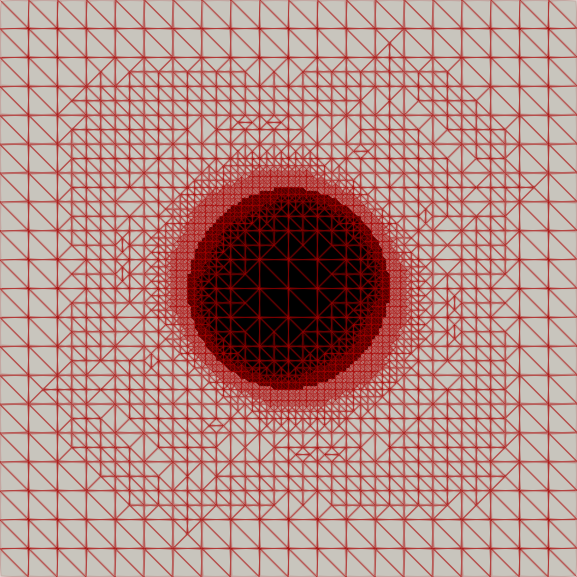
\includegraphics[width=0.32\textwidth]{static/sphereudo.png} \, 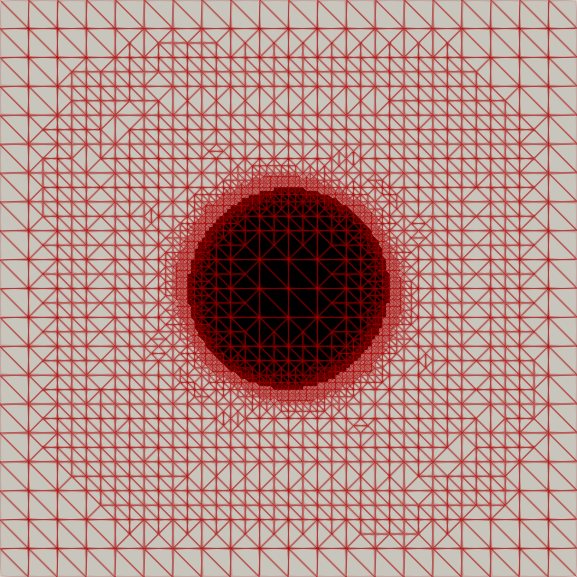
\includegraphics[width=0.32\textwidth]{static/spherevcd.png} \,\,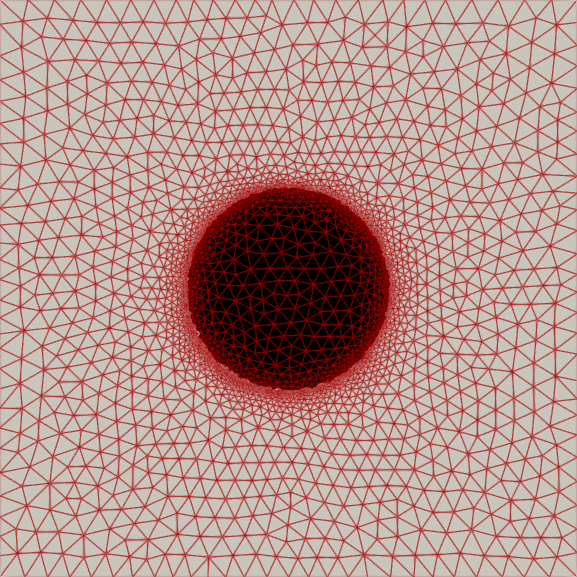
\includegraphics[width=0.32\textwidth]{static/sphereavm.png}}
\caption{Meshes computed from the UDO (left; see also Figure \ref{fig:ball}), VCD (middle), and AVM (right) methods.}
\label{fig:threeballmeshes}
\end{figure}

Example meshes are shown in Figure \ref{fig:threeballmeshes}.  They were generated by 3 levels of refinement using the above three methods, starting from a coarse uniform mesh, on the obstacle problem shown in Figures \ref{fig:ball} and \ref{fig:activesizes} (middle).  These AMR methods increase the resolution both near the free boundary and in the inactive set.

Our numerical results in Sections \ref{sec:results} and \ref{sec:app}, from the three strategies, will justify our somewhat-heuristic approach to AMR for VIs.  Because the convergence of VI problems is dominated by the error in approximating the free boundary, an AMR scheme that quickly concentrates effort around an accurately-computed free boundary, possibly augmented by PDE-type error estimators in the inactive set (Section \ref{sec:aposteriori}), will accelerate convergence and reduce unnecessary computation.

AMR for VI problems has been preliminarily explored in the literature.  The first published analysis may be \cite{AinsworthOdenLee1993}, giving an error bound for the classical obstacle problem in terms of local functionals associated with each element.  The monograph by Suttmeier \cite{Suttmeier2008} covers a broader class of problems, including elasticity.  For the classical obstacle problem, the constructable error estimators in these works require heuristic assumptions which may not hold in general.  (See inequality (42) in \cite{AinsworthOdenLee1993}, and the approximation ``$(u-\psi)\lambda_h\approx 0$'' in \cite{Suttmeier2008}.)  To our knowledge these approaches are not found in publicly-available implementations, nor are they as efficient, for computing high-resolution approximations to free boundaries, as the best of our strategies.

Our focus in this paper is on AMR performance, but not solver performance.  We use a fixed, VI-adapted, reduced-space Newton method with line search \cite{BensonMunson2006}, implemented in PETSc \cite{petsc-user-ref}, for all examples.  Note that since the constraint $u \geq \psi$ makes VI problems nonlinear, even if the operator is linear, an iterative solver like Newton is required.  Such a numerical method cannot converge quadratically until the active and inactive sets stabilize on the given mesh, equivalently once the discrete free boundary is identified.  At that point convergence can occur in one additional iteration, for a linear operator, or otherwise in a few iterations for well-behaved nonlinear operators.  Such a reduced-space Newton solver can only adjust the approximated free boundary by one-cell per iteration \citep{GraeserKornhuber2009}, and thus overall convergence becomes proportional to the number of grid spaces between the initial-iterate and final free boundaries on the mesh \citep{Bueler2021}.

VI solver performance can be substantially improved by combining the AMR meshing strategies here with a multilevel approach.  The solver in \cite{BuelerFarrell2024}, for example, uses coarse meshes to make large geometrical corrections in the free boundary.  This path, which promises highly-scalable solutions of obstacle problems, is for future research.

In summary, here are two principles of the AMR methods of this paper:
\renewcommand{\labelenumi}{\arabic{enumi}.}
\begin{enumerate}
\item Relative to uniform refinement, the methods exhibit significant improvements in error norm convergence.  This is measured by norm or free-boundary localization (geometrical) error per mesh degree of freedom.
\item Their implementations (\href{https://github.com/StefanoFochesatto/VI-AMR}{{\small \texttt{github.com/StefanoFochesatto/VI-AMR}}}), which extend the widely-distributed Firedrake \cite{Langeetal2016} FE library, are parallel, well-documented, and easy-to-use.
\end{enumerate}

The paper is organized as follows:  Table \ref{tab:abbrev} gives the few abbreviations used herein.  Section \ref{sec:vifem} provides \emph{a priori} norm bounds for FE methods applied to VI problems.  Section \ref{sec:aposteriori} addresses \emph{a posteriori} error estimators which can be applied in the inactive set, and it identifies problems where active-set refinement can be avoided.  Section \ref{sec:viamr} describes the three methods in more detail.  Sections \ref{sec:results}--\ref{sec:conclusion} compare and discuss the performance of these AMR algorithms on model problems, and on a realistic glacier application.

\begin{table}[ht]
\centering
\begin{minipage}[t]{0.45\textwidth}
\vspace{0pt}
{\small
\begin{tabular}{ll} \\
AMR       & adaptive mesh refinement \\
AVM$^*$   & averaged-metric \\
BR        & Babu\v{s}ka--Rheinboldt \\
CG        & continuous Galerkin \\
DAG       & directed acyclic graph \\
DG        & discontinuous Galerkin \\
DWR       & dual-weighted residual
\end{tabular}
}
\end{minipage}
\quad
\begin{minipage}[t]{0.45\textwidth}
\vspace{0pt}
{\small
\begin{tabular}{ll} \\
FE        & finite element \\
GR        & gradient recovery \\
PDE       & partial differential equation \\
SBR       & skeleton-based refinement \\
UDO$^*$   & unstructured dilation operator \\
VCD$^*$   & variable-coefficient diffusion \\
VI        & variational inequality
\end{tabular}
}
\end{minipage}


\caption{Abbreviations used in this paper.  Stars indicate the new AMR methods.}
\label{tab:abbrev}
\end{table}


\section{Variational inequalities and their finite element approximations} \label{sec:vifem}

We start with the VI formulation of unilateral obstacle problems in Banach spaces.  Consider a bounded, open domain $\Omega \subset \RR^d$, $d=2,3$, with Lipschitz boundary \cite{Ciarlet2002}.  We assume that $\Omega$ is polygonal or polyhedral.  Let $\cX = W^{1,p}(\Omega)$, $p>1$, be the Sobolev space of measurable functions with $p$th-integrable gradients \cite{Evans2010}.  We will assume continuous problem data, allowing well-defined point values, so suppose $\psi \in \cX \cap C(\bar\Omega)$ and $g\in C(\partial \Omega)$ satisfy $g \ge \psi|_{\partial\Omega}$.  Define the admissible subset
\begin{equation} \label{eq:admissible}
\cK = \{v \in \cX \,:\, v \ge \psi \text{ and } v|_{\partial \Omega} = g\},
\end{equation}
as for \eqref{eq:classical:admissible}.  Note that $\cK\subset \cX$ is closed and convex.  Observe that generally $\psi\notin\cK$.

Let $\cX'$ be the dual space of $\cX$, with the application of $\omega \in \cX'$ to $v\in \cX$ denoted $\omega[v] \in \RR$.  The norm on $\cX$ is denoted $\|\cdot\|$, while for $\cX'$ it is $\|\omega\|' = \sup_{\|v\|=1} |\omega[v]|$.  Let $F:\cK \to \cX'$ be a given operator, generally nonlinear, and let $\ell\in \cX'$ be given.  The VI associated to this data, a unilateral obstacle problem, is to find $u\in \cK$ so that
\begin{equation} \label{eq:vi}
F(u)[v - u] \ge \ell[v - u] \quad \text{ for all } v \in \cK.
\end{equation}

Our VI problems can be analyzed within the framework of coercivity and Lipschitz continuity.  We say $F$ is $q$-coercive, $1<q<\infty$, if there is $\alpha>0$ so that
\begin{equation} \label{eq:coercive}
(F(v) - F(w))[v - w] \ge \alpha \|v-w\|^q
\end{equation}
for all $v,w \in \cK$.  Note that if $F$ is $q$-coercive then it is also strictly monotone: $(F(v) - F(w))[v - w] > 0$ for $v\ne w$.  Let $B_R(0)$ be the origin-centered open ball in $\cX$ of radius $R>0$.  We say $F$ is Lipschitz on bounded subsets if there is $C(R)>0$ so that
\begin{equation} \label{eq:lipschitz}
\|F(v)-F(w)\|' \le C(R) \|v-w\|
\end{equation}
for all $v,w \in B_R(0)\cap \cK$.  If $F$ satisfies \eqref{eq:lipschitz} then it is continuous.

From the coercivity, strict monotonicity, and continuity of $F$ it follows that a unique solution to \eqref{eq:vi} exists \cite[Corollary III.1.8]{KinderlehrerStampacchia1980}.

\begin{example}  \label{example:classicalobstacle}
In the classical obstacle problem \eqref{eq:classical:vi}, over $\cX=H^1(\Omega)=W^{1,2}(\Omega)$,
\begin{equation} \label{eq:classical:bilinearform}
F(u)[v] = a(u,v) = \int_\Omega \grad u\cdot \grad v\,dx
\end{equation}
is in fact bilinear.  It is $2$-coercive because the Laplacian is uniformly elliptic \cite{Evans2010}, and it is Lipschitz over $\cX$ with constant $C=1$.
\end{example}

While $F$ in Example \ref{example:classicalobstacle} is defined on all of $\cX$, the general operator $F$ in \eqref{eq:vi} might be only defined on $\cK$.  Section \ref{sec:app} provides such an example.

Note that if the inequality constraint in \eqref{eq:vi} were absent then the residual would be zero almost everywhere ($F(u)-\ell=0$); this is the PDE case.  However, for a VI, over $\cK$ defined by \eqref{eq:admissible}, we only have that $F(u)-\ell=0$ a.e.~within the unknown inactive set $I_u$.  In fact, the residual $F(u)-\ell\in \cX'$ might be highly-irregular in the active set $A_u$, but it is at least nonnegative.  The following lemma states the (weak) complementarity property associated to VI \eqref{eq:vi}; compare strong-form complementarity \eqref{eq:classical:ncp} for \eqref{eq:classical:vi}.

\begin{lemma} \label{lem:measure}\cite[Theorem II.6.9]{KinderlehrerStampacchia1980}.  Suppose $u\in \cK$ solves \eqref{eq:vi}.  Then $F(u)-\ell=d\mu_u$ is a positive Radon measure supported in the active set $A_u$.  Thus for $w\in\cX$ we have
\begin{equation}
(F(u)-\ell)[w] = \int_{A_u} w\, d\mu_u. \label{eq:measure}
\end{equation}
\end{lemma}

Now let $\cT_h$ be a shape-regular mesh partition (triangulation, etc.) of $\Omega$ \cite{AinsworthOden2000,ElmanSilvesterWathen2014}.  Let $\cX_h \subset \cX \cap C(\bar\Omega)$ be a conforming finite-dimensional FE subspace over $\cT_h$.  (Our examples will be piecewise-linear: $\cX_h=P_1$.)  Assume that there is $g_h\in\cX_h$ such that $g_h=g$ exactly along $\partial \Omega$.  Let $\psi_h \in \cX_h$ be the FE obstacle, which satisfies the compatibility requirement $\psi_h \le g_h$ along $\partial\Omega$; note that no other requirement, for now, relates $\psi_h$ to $\psi$.  Define the (nonempty) FE admissible set
\begin{equation} \label{eq:fe:admissible}
\cK_h = \{v_h \in \cX_h \,:\, v_h \ge \psi_h \text{ and } v_h|_{\partial \Omega} = g_h|_{\partial\Omega}\}.
\end{equation}
Our FE method seeks $u_h\in\cK_h$ satisfying the VI problem
\begin{equation} \label{eq:fe:vi}
F(u_h)[v_h - u_h] \ge \ell[v_h - u_h] \quad \text{ for all } v_h \in \cK_h.
\end{equation}
The same argument given for \eqref{eq:vi} shows that \eqref{eq:fe:vi} has a unique solution $u_h$.  Define
\begin{equation}
  I_u^h = \{x \in \Omega \,:\, u_h(x) > \psi_h(x)\}, \quad A_u^h = \Omega \setminus I_u^h, \label{eq:fe:sets}
\end{equation}
the numerical inactive and active sets, respectively, defined \emph{a posteriori} from the solution to \eqref{eq:fe:vi}.

Because $\cK_h \subset \cX_h \subset \cX$, we may regard \eqref{eq:fe:vi} as a conforming FE method for \eqref{eq:vi}.  However, this is subtle for an obstacle problem, depending on the relationship between $\psi$ and $\psi_h$.  If $\psi_h$ is an interpolant of $\psi$, $\psi_h = \Pi_h \psi$, then $\cK_h \approx \cK$ in some sense, but one may state three precise levels of ``conforming admissibility'':
\renewcommand{\labelenumi}{\emph{\roman{enumi})}}
\begin{enumerate}
\item $\cK_h \not \subset \cK$
\item $\cK_h \subset \cK$
\item $\cK_h = \cK \cap \cX_h$
\end{enumerate}
As noted early-on by Ciarlet \cite[Figure 5.1.3]{Ciarlet2002}, situation \emph{i)} generally applies for an interpolated obstacle $\psi_h = \Pi_h \psi$, e.g.~for $\cX_h=P_1$ and when $\psi$ is not convex.  Situation \emph{ii)} holds when $\psi_h \ge \psi$, which can be imposed by using a monotone injection operator, e.g.~``$\psi_h = R^\oplus \psi$'' in the notation from \cite{BuelerFarrell2024}.  (For related ideas, see the proof of Theorem 5.1.2 in \cite{Ciarlet2002}, and \cite{GraeserKornhuber2009}.)  The strongest condition \emph{iii)} holds if $\psi_h=\psi$ exactly, for example when $\psi=0$ in the porous dam problems considered by \cite{AinsworthOdenLee1993}.

Note that the obstacle $\psi$ is given \emph{as data} for VI problem \eqref{eq:vi}.  Point values of $\psi$ can therefore be evaluated as desired to represent (improve) $u_h$ within the numerical active set $A_u^h$.  That is, over elements where there is believed to be active-set agreement, i.e.~$K\in\cT_h$ such that $K \subset A_u \cap A_u^h$, reducing the error $e=u-u_h=\psi-u_h$ can be addressed in post-processing simply by evaluating the data $\psi$.  By contrast, improvement of the mesh, and re-solution of the FE problem, is needed to more-accurately locate the free boundary and reduce $\|e\|$.  Convergence also requires more-accurate FE solution within the inactive set, e.g.~using mesh refinement.  However, refinement deeper within a stabilized active set may be wasted effort.

The following \emph{a priori} theorem, which bounds the norm of $e=u-u_h$, generalizes Falk \cite{Falk1974}; see also Theorem 5.1.1 in \cite{Ciarlet2002}.  In applying it we will distinguish between numerical errors arising from mis-locating the exact free boundary, thus mis-identifying the exact active and inactive sets, versus the question of accurate approximation of the original obstacle $\psi$ within the active set.

\begin{theorem} \label{thm:genfalk}  For $1<q<\infty$, define the conjugate exponent $q'=q/(q-1)$.  Assume that $F$ is $q$-coercive and Lipschitz on bounded sets of its domain.  Suppose $u\in\cK$ solves \eqref{eq:vi} and $u_h\in\cK_h$ solves \eqref{eq:fe:vi}.  Let $R_h=\max\{\|u\|,\|u_h\|\}$.  Then there is a constant $c(R_h)>0$, not otherwise depending on $u$ or $u_h$, so that
\begin{align}
\|u-u_h\|^q &\le \frac{2}{\alpha} \bigg( \inf_{v\in\cK} \int_{A_u} (v-u_h)\,d\mu_u \label{eq:falk} \\
   &\qquad\quad + \inf_{v_h\in\cK_h} \int_{A_u} (v_h-\psi)\,d\mu_u \notag \\
   &\qquad\quad + c(R_h) \inf_{v_h\in\cK_h} \|v_h - u\|^{q'}\bigg). \notag
\end{align}
\end{theorem}

\begin{proof}  For arbitrary $v\in\cK$ and $v_h\in\cK_h$, rewrite \eqref{eq:vi} and \eqref{eq:fe:vi} as $F(u)[u] \le F(u)[v] + \ell[u-v]$ and $F(u_h)[u_h] \le F(u_h)[v_h] + \ell[u_h-v_h]$, respectively.  It follows from these inequalities, and $q$-coercivity of $F$, that
\begin{align}
\alpha \|u-u_h\|^q &\le \left(F(u)-F(u_h)\right)[u-u_h] \label{eq:falkdance} \\
  &= F(u)[u] + F(u_h)[u_h] - F(u)[u_h] - F(u_h)[u] \notag \\
  &\le F(u)[v] + \ell[u-v] + F(u_h)[v_h] + \ell[u_h-v_h] \notag \\
  &\qquad - F(u)[u_h] - F(u_h)[u] \notag \\
  &= F(u)[v-u_h] - \ell[v-u_h] + F(u_h)[v_h-u] - \ell[v_h-u] \notag \\
  &= \left(F(u)-\ell\right)[v-u_h] + \left(F(u)-\ell\right)[v_h-u] \notag \\
  &\qquad + \left(F(u)-F(u_h)\right)[u-v_h] \notag
\end{align}
Since $u,u_h\in B_{R_h} = \{w\in\cX\,:\,\|w\|\le R_h\}$, by the Lipschitz assumption \eqref{eq:lipschitz} there is $C(R_h)>0$ so that the last term from \eqref{eq:falkdance} has bound
\begin{equation}
\left(F(u)-F(u_h)\right)[u-v_h] \le C(R_h) \|u-u_h\|\|u-v_h\|. \label{eq:falklip}
\end{equation}
Now use Young's inequality with $\eps>0$ \cite[Appendix B.2]{Evans2010} on \eqref{eq:falklip}.  We have:
\begin{align}
\alpha \|u-u_h\|^q &\le \left(F(u)-\ell\right)[v-u_h] + \left(F(u)-\ell\right)[v_h-u]  \label{eq:falkyoung} \\
  &\qquad + C(R_h) \left(\eps\|u-u_h\|^q + \tilde C(\eps) \|u-v_h\|^{q'}\right) \notag
\end{align}
where $\tilde C(\eps) = (\eps q)^{-q'/q} {q'}^{-1}$.  Choose $\eps>0$ so that $C(R_h) \eps \le \alpha/2$.  Then
\begin{align}
\frac{\alpha}{2} \|u-u_h\|^q &\le \left(F(u)-\ell\right)[v-u_h] + \left(F(u)-\ell\right)[v_h-u]  \label{eq:falkalmost} \\
  &\qquad + C(R_h) \tilde C(\eps) \|u-v_h\|^{q'} \notag
\end{align}
Apply Lemma \ref{lem:measure} to \eqref{eq:falkalmost}, note $u=\psi$ a.e.~in $A_u$, and take infimums to show \eqref{eq:falk}.\end{proof}

Theorem \ref{thm:genfalk} can be extended to non-conforming operators $F_h\approx F$ by adding a fourth term ``$(F(u_h)-F_h(u_h))[u_h]$'' to the bound \cite[Theorem 6.3]{Bueler2024}.  However, we will not need this extended result.

In situation \emph{ii)} earlier, namely $\cK_h\subset \cK$, the first ``$\inf$'' term from \eqref{eq:falk} is zero.

\begin{corollary} \label{cor:falkconforming}
Suppose $\cK_h\subset \cK$, plus the other hypotheses of Theorem \ref{thm:genfalk}.  Then
\begin{equation} \label{eq:falkconforming}
\|u-u_h\|^q \le \frac{2}{\alpha} \left(\inf_{v_h\in\cK_h} \int_{A_u} (v_h-\psi)\,d\mu_u + c(R_h) \inf_{v_h\in\cK_h} \|v_h - u\|^{q'}\right).
\end{equation}
\end{corollary}

Furthermore, in the unconstrained PDE case, where $A_u=\emptyset$ and $d\mu_u=0$, the bound can be reduced to Cea's lemma for $q$-coercive operators, namely $\|u-u_h\| \lesssim \inf_{v_h\in\cK_h} \|v_h - u\|^{1/(q-1)}$.  In any case, as is standard in FE theory, $\inf_{v_h\in\cK_h} \|v_h - u\|$ can be addressed by a regularity theory for the exact solution $u$, plus interpolation theory \cite{AinsworthOden2000,ElmanSilvesterWathen2014}, yielding convergence \cite[Theorem 5.1.2]{Ciarlet2002}.

However, how should we interpret the $\cK_h$ infimum term in \eqref{eq:falk} and \eqref{eq:falkconforming}?:
	$$(\ast) \qquad \inf_{v_h\in\cK_h} \int_{A_u} (v_h-\psi)\,d\mu_u$$
This is unrelated to the FE solution $u_h$.  If $v_h < \psi$ is locally possible then $(\ast)$ might be negative, but then situation \emph{i)} holds and the ``$\inf_{v\in\cK}$'' term in \eqref{eq:falk} might counter-act (i.e.~if $v\ge \psi > u_h$ anywhere).  In the simpler situation \emph{ii)}, where $\psi_h\ge \psi$ and $\cK_h\subset \cK$, the term is at least nonnegative.  It might be large because no $v_h\in\cK_h$ is close to $\psi$ over $A_u$, for instance where $v_h\ge \psi_h \gg \psi$.  On the other hand, $(\ast)$ might be large even where $v_h-\psi$ can be made small over $A_u$, that is, if the source functional $\ell$ causes the residual $F(u)-\ell\ge 0$ to be large in $A_u$.  (Meaning: $d\mu_u(S)$ is positive and large for some measurable $S\subset A_u$.)  In summary, in the situation where $\cK_h\subset \cK$, the bound \eqref{eq:falkconforming} is significantly larger than that from Cea's lemma only when the FE functions $v_h$ are blocked by $\psi_h$ from descending close to the continuum obstacle $\psi$, or when the (exact) residual $d\mu_u$ is large in the (exact) active set $A_u$, or both.


\section{\emph{A posteriori} error estimation in inactive and active sets} \label{sec:aposteriori}

For $u\in\cX$ solving VI \eqref{eq:vi}, a PDE holds in the inactive set $I_u$, the so-called \emph{interior condition} \cite{KinderlehrerStampacchia1980}.  In Section \ref{sec:results} we will demonstrate strategies which primarily do (\emph{a posteriori}) refinement in the geometric vicinity of the free boundary, but we also exploit \emph{a posteriori} error indicators for the interior condition PDE.

We consider two indicators, the first of which is well-defined independent of that PDE.  It is based on \emph{gradient recovery} (GR) \cite[Chapter 4]{AinsworthOden2000}, and it is used in Section \ref{sec:app}.

\begin{example}  \label{example:gradrecovery}  Suppose $\cX_h$ is a continuous, piecewise-polynomial FE space, of degree $p$, and suppose $u_h\in\cX_h$.  Generally $\grad u_h$ is discontinuous, but it is well-defined on each element.  Let $\cY_h$ be the (scalar) discontinous space with polynomial degree $p-1$, so $\grad u_h \in \cY_h^d$.  Suppose there is a linear operator $G : \cY_h^d \to \cX_h^d$, which we call \emph{gradient recovery}, which is designed so that $G(u_h)\approx \grad u$ in $\cX^d$ in some sense, assuming of course that $u_h\approx u$ in $\cX$.  Then the error indicator $\eta_K\ge 0$ for this GR method, over an element $K \in\cT_h$, is
\begin{equation} \label{eq:gradrecoveryindicator}
\eta_K^2 = \int_K \left|G(u_h) - \grad u_h\right|^2.
\end{equation}
\end{example}

Generally one applies the indicator to a solution $u_h \in \cK_h$ of \eqref{eq:fe:vi}, but observe that formula \eqref{eq:gradrecoveryindicator} is well-defined for any $u_h \in \cX_h$.  Let $\eta^2 = \sum_{K\in\cT_h} \eta_K^2$.  For certain gradient recovery methods $G$ it can be shown that, at least for the Poisson equation, $\eta \sim |u-u_h|_{H^1}$ (energy norm) asymptotically as $h\to 0$ \cite[Theorem 4.4]{AinsworthOden2000}.

In Sections \ref{sec:results} and \ref{sec:app} our GR operation will simply use orthogonal projection in $L^2$.  That is, $w = G(u_h) \in \cX_h^d$ is the minimizer of
\begin{equation} \label{eq:gradrecoveryprojection}
J(w) = \int_\Omega |w - \grad u_h|^2\,dx.
\end{equation}
In the results shown later, the space $\cX_h$ will be the continuous $P_1$ FE space, thus $\grad u_h$ is in (vector-valued) discontinuous $P_0$ space.  It is not clear to the current authors whether Theorem 4.4 in \cite{AinsworthOden2000} applies to our recovery operator.  (The operators analyzed by \cite{AinsworthOden2000} act by averaging element centroid values to get $\cX_h$ nodal values.)

The second indicator is only stated for the classical obstacle problem.  It is a well-known \emph{explicit error estimator} for the Poisson equation \cite[Chapter 2]{AinsworthOden2000}.

\begin{example}  \label{example:br}  Suppose $u \in H^1(\Omega)$ solves the weak form PDE $a(u,v) = \int_\Omega f v\,dx$ for all $v \in H^1_0(\Omega)$, with $u=g$ on $\partial \Omega$, for the bilinear form $a(u,v)=\int_\Omega \grad u\cdot \grad v\,dx$.  Suppose that $u_h$ from the continuous, $P_1$ FE space $\cX_h$ solves the corresponding finite-dimensional weak form.  For each element $K \in \cT_h$, define $n_K$ as the unit outward normal vector on $\partial K$.  For a pair of elements $L,K$ incident to an edge $\gamma$, and any vector field $Z$ with traces $Z_L,Z_K$ on $\gamma$, let $\left\llbracket Z \cdot n \right\rrbracket = Z_L \cdot n_L + Z_K \cdot n_K$ be the jump of $Z$ on $\gamma$.  Given the Poisson (strong) residual $r(v)=-\nabla^2 v - f$ defined within the elements, the Babu\v{s}ka--Rheinboldt (BR) \cite{BabuskaRheinboldt1979} error estimator is
\begin{equation} \label{eq:brestimator}
\eta_K^2 = h_K^2 \int_K |r(u_h)|^2\,dx + \frac{h_K}{2} \sum_{\gamma \in \partial K \setminus \partial \Omega} \int_{\gamma} \left\llbracket \grad u_h \cdot n \right\rrbracket^2\,dS,
\end{equation}
where $h_K$ is the diameter of $K$.  It can be shown \cite[Chapter 2]{AinsworthOden2000} that the energy error is bounded by the sum of these indicators:
\begin{equation} \label{eq:brbound}
|u-u_h|_{H^1}^2 = \int_\Omega |\grad(u-u_h)|^2\,dx \le C \eta^2,
\end{equation}
where $\eta^2 = \sum_{K\in\cT_h} \eta_K^2$.  The constant $C>0$ is determined by the element-wise and edge-wise approximation properties of the elements, including shape regularity.  The $L^2$ error can be bounded by a similar indicator (estimator) \cite[Section 2.4]{AinsworthOden2000}, which replaces the powers in \eqref{eq:brestimator} by $h_K^4,h_K^3$, respectively.
\end{example}

Whether $\eta_K$ is computed as in Example \ref{example:gradrecovery} or \ref{example:br}, we will treat these values as local element-wise error estimators.  That is, the set of values $\eta_K$ will be thresholded to providing tagging of elements for refinement; see \cite[Section 4.2]{BangerthRannacher2003} for discussion of such techniques.  Specifically, all (computed) inactive elements satisfying $\eta_K \ge \theta \max \eta_K$, for $0<\theta<1$, will be tagged and refined.  For more details see the next Section.

The BR error estimator in Example \ref{example:br}, for the Poisson equation, is explicit and easily-computed.  Ainsworth, Oden, and Lee \cite{AinsworthOdenLee1993} extend this estimator to certain obstacle problems, but with heuristic aspects.

For PDE problems, an alternative to a local BR-type estimator is provided by the \emph{dual weighted residual} (DWR) technique \cite{BangerthRannacher2003}.  Such estimators are defined using a particular quantity of interest and nonlocal weights (approximately) computed from an adjoint problem.  The weights are essentially Green's functions of the adjoint PDE.  Suttmeier \cite{Suttmeier2008} has extended this DWR technique to VI problems, but this also requires heuristic steps even for the classical obstacle problem.  However, at least for obstacle problems with disconnected inactive sets---see Figure \ref{fig:activesizes} (right)---the weightings from a DWR technique are zero when a free boundary separates the components of the inactive set.  Even if the inactive set is connected, the weights in DWR would be very small in a problem like the one with a spiral active set (Figure \ref{fig:activesizes}, left); though the inactive set is connected it is geometrically very complicated.

In this paper we avoid the complexity of the techniques in references \cite{AinsworthOdenLee1993} and \cite{Suttmeier2008}, and instead take a more pragmatic approach.  We apply fast (and again heuristic) refinement near a computed free boundary.  We combine this with application of a gradient-recovery or BR estimator, as above, within the computed inactive sets.

Returning to the general, continuum problem \eqref{eq:vi}, next we point out a qualitative property of certain unilateral obstacle problems, which can be exploited \emph{a posteriori} in the active set.  Note that for the classical obstacle problem \eqref{eq:classical:vi}, assuming a continuous source $f\in C(\bar\Omega)$ for simplicity, in general an upward force $f(x)>0$ can occur in the active set.  That is, the force, while locally upward, may be insufficient to lift $u$ above a concave $\psi$.  However, in certain obstacle problems this cannot occur.

\begin{lemma} \label{lem:blister}
Suppose that $\psi=0$ and $\ell[v] = \int_\Omega fv\,dx$ for $f\in C(\bar\Omega)$.  Suppose also that $F$ is given by measurable densities, for example $F(w)[v]=\int_\Omega \phi(w(x),\grad w(x)) v(x) + \Phi(w(x),\grad w(x)) \cdot \grad v(x)\,dx$, satisfying $\phi(0,0)=0$ and $\Phi(0,0)=0$.  Then for $u$ solving \eqref{eq:vi}, $f\le 0$ a.e.~in $A_u$.
\end{lemma}

\begin{proof}
Let $S\subset A_u$ be a Borel set, and denote its indicator function by $\chi_S \in L^\infty(\Omega)$.  The operator value $F(u)[\chi_S]$ is well-defined, \emph{and zero}, because $S$ is in the active set, by a density argument.  Thus by Lemma \ref{lem:measure},
\begin{equation*}
0 \le d\mu_u(S) = F(u)[\chi_S]-\ell[\chi_S] = 0 - \ell[\chi_S] = -\int_S f\,dx.
\end{equation*}
This shows $f\le 0$ a.e.~with respect to Lebesgue measure.
\end{proof}

The hypotheses of the Lemma clearly hold for problem \eqref{eq:classical:vi} if $\psi=0$.

By definition, we say that a unilateral obstacle problem, based on $\ell[v] = \int_\Omega fv\,dx$ with $f\in C(\bar \Omega)$, has the \emph{blistering property} if $A_u \subset \{x \in \Omega\, :\, f(x)\le 0\}$ \cite{JouvetBueler2012}, up to a set of measure zero, that is, if the conclusion of Lemma \ref{lem:blister} holds.  To explain the language, if $f(x)>0$ anywhere, for continuous $f$, then under this property the inactive set $I_u$ must be non-empty, and $x\in I_u$; even a small upward force ``blisters'' the membrane off the obstacle.  Note that porous-dam saturation free boundary problems, such as the examples in \cite{AinsworthOdenLee1993}, have this property because $\psi=0$.

In fact, any classical problem \eqref{eq:classical:vi} with a smooth obstacle $\psi\in C^2(\bar\Omega)$ can be transformed into one with the blistering property.  To see this, make the obstacle zero by transforming $\tilde v=v-\psi$, thus $\tilde\cK = \{\tilde v\in\cX\,:\,\tilde v\ge 0 \text{ and } \tilde v|_{\partial\Omega}=g-\psi|_{\partial\Omega}\}$.  Integration-by-parts shows \eqref{eq:classical:vi} is equivalent to finding $\tilde u = u -\psi \in \tilde \cK$ so that
\begin{equation} \label{eq:classical:vi:blister}
\int_\Omega \nabla \tilde u \cdot \nabla(\tilde v - \tilde u) \ge \int_\Omega \left(f+\grad^2\psi\right)(\tilde v - \tilde u) \quad \text{ for all } \tilde v \in \tilde \cK.
\end{equation}
For VI problem \eqref{eq:classical:vi:blister}, if $x\in A_{\tilde u} = \{\tilde u(x)=0\}$ then $\tilde f(x)= f(x)+\grad^2\psi(x)\le 0$.

For blistering-property problems, substantial AMR efficiency can be achieved by avoiding refinement in the computed active set $A_u^h$.  However, one must carefully identify those elements where no refinement would be beneficial.  Assume the blistering property, and consider an element $K\in \cT_h$ in the active set $A_u^h$.  (In our implementation, this means that \emph{every node in the closure of $K$} is active, according to a tolerance criterion.)  The degenerate case $f=0$ must first be excluded within $K$.  That is, one must know that $K$ is contained in the set $\Omega_- = \{x\in \Omega\,:\,f(x) < 0\}$, which is a property of the data of the problem.  If later refinements might move the free boundary to impinge on $K$ then refinement of $K$ would be appropriate, thus our techniques (next Section) will be designed to mark for refinement those active-set elements which are ``near'' $\Gamma_u^h$ in some sense.  However, if $f \le 0$ on $K$, and if $K$ is too far from the free boundary to be inactivated by later solutions along the refinement path, then $K$ can remain unrefined without affecting solution accuracy.


\section{New adaptive mesh refinement strategies} \label{sec:viamr}

Our first two methods for adaptive mesh refinement (AMR) for VIs, namely Algorithms \ref{alg:udo} and \ref{alg:vcd} below, are of \emph{tag-and-refine} type.  Later in this section we compare them to a third, more-expensive \emph{metric-based mesh adaptation} approach \cite{Wallworketal2020}, which can hold the mesh complexity approximately constant.

These methods start from a computed solution to FE VI problem \eqref{eq:fe:vi}.  We need only the mesh $\cT_h$, the obstacle $\psi_h \in \cX_h$, and the admissible solution $u_h \in \cK_h \subset \cX_h$.  The following two concepts are fundamental.

\begin{definition} \label{def:nodalactive}
Denote the vertices of $\cT_h$ by $x_j$.  Given $u_h \ge \psi_h$ and a tolerance $\text{tol}>0$, the \emph{(a posteriori) nodal active set indicator} is the function $\nu_h\in\CG_1(\cT_h)$ satisfying
	$$\nu_h(x_j) = \begin{cases} 1, & u_h(x_j) - \psi_h(x_j) < \text{tol} \\
	                             0, & \text{otherwise}\end{cases}$$
\end{definition}

\begin{definition} \label{def:marking}
An \emph{element marking} (\emph{tagging}) of a mesh $\cT_h$ is a piecewise-constant indicator function $I_h \in \DG_0(\cT_h)$ with values in $\{0,1\}$.  Elements $K \in \cT_h$ such that $I_h|_K=1$ will be refined.
\end{definition}

For PDE problems, an element marking is typically derived from an error estimator $\eta_K$ associated with a quantity of interest, such as energy or $L^2$ norm error, or a local functional \cite{BangerthRannacher2003}.  (For the interior condition of problem \eqref{eq:vi}, we gave examples in Section \ref{sec:aposteriori}.)  However, a primary quantity of interest for obstacle problems is \emph{vicinity to the unknown free boundary}.  We do not associate this concept with a precise functional, but instead Algorithms \ref{alg:udo} and \ref{alg:vcd} proceed heuristically to convert an \emph{a posteriori} nodal active set indicator $\nu_h$ (Definition \ref{def:nodalactive}) into an element marking $I_h$ (Definition \ref{def:marking}), with the goal of improving the approximation of the free boundary.

From the marking $I_h$ we then apply \emph{skeleton-based refinement} (SBR) \cite{PlazaCarey2000} to generate a refined mesh with no hanging nodes and good mesh quality.  Note that two implementations of SBR are available to Firedrake applications, namely from the DMPlex component of PETSc \cite{petsc-user-ref} or the Netgen library \cite{Betteridgeetal2024}; only the latter is (currently) capable of 3D refinement.  In fact, the use of DMPlex queries is essential to Algorithm \ref{alg:udo} below, so let us sketch aspects of how this domain management class supports unstructured meshes \cite{Langeetal2016}.  A DMPlex object stores the topology (connectivity of entities) of a $d=1,2,3$ FE mesh.  (The mesh geometry is in an associated PetscSection object for the vertex coordinates.)  Every mesh entity, regardless of dimension, is assigned a unique index.  Mesh connectivity can be understood as a stratified directed acyclic graph (DAG) in which a covering (incidence) relationship between mesh entities determines the directed edges.  For example, a triangle within a 2D mesh is covered by its three edges, each of which is covered by its two endpoints (vertices).  Each stratum in the DAG represents a dimensional class of mesh entity.  For example the cells, edges, and vertices in a 2D mesh are at strata indices (``height'') of $0$, $1$, and $2$ respectively.  Given the index $p$ of a mesh entity, we will use the following DMPlex mesh topology queries \cite{petsc-user-ref}:  The operation $\text{\emph{cone}}(p)$ returns the indices of all entities which cover entity $p$.  Its dual, which returns all the entities which are covered by $p$, is $\text{\emph{support}}(p)$.  The transitive closure of \emph{cone} is $\text{\emph{closure}}(p)$, and that of \emph{support} is $\text{\emph{star}}(p)$.  In our application we need only the indices of vertices in the element closure; we denote this $\text{\emph{closure}}^\wedge(k)$.  Similarly, $\text{\emph{star}}_\vee(j)$ extracts only element indices in the vertex star.

With this preparation we can state the Unstructured Dilation Operator (UDO) method, Algorithm \ref{alg:udo}.  It first computes a nodal active set indicator $\nu_h$ (Definition \ref{def:nodalactive}).  Denoting the degrees of freedom in $\DG_0(\cT_h)$ by $x_k$, it finds the set of indices $k$ of elements $K\in\cT_h$ such that $0<\nu_h(x_k)<1$.  This condition holds when at least one of the vertices incident to $K$ is in the active set (according to $u_h$), and at least one is not.  Then the method alternates closure and star on the element set $n$ times, expanding it by $n$ elements, and then generates the element marking $I_h$ (Definition \ref{def:marking}).

\begin{algorithm}[ht]
	\caption{Unstructured Dilation Operator (UDO) element marking}
	\begin{algorithmic}[1]
		\Require mesh $\cT_h$, solution $u_h \in \cK_h$, obstacle $\psi_h \in \cX_h$, tolerance $\text{tol} > 0$, and neighborhood expansion parameter $n\ge 1$.
		\State Compute nodal active set indicator $\nu_h \in \CG_1(\cT_h)$.
		\State Find initial element index set $S_0$: \,$k\in S_0$ if $\nu_h(x_k) \in (0,1)$.
		\For{$i=0,\dots,n-1$}
		    $$S_{i+1} = \bigcup_{k\in S_i}\, \bigcup_{j\in \text{\emph{closure}}^\wedge(k)} \text{\emph{star}}_\vee(j)$$
		\EndFor \\
		\Return marking $I_h \in \DG_0(\cT_h)$ of all elements in $S_n$.
	\end{algorithmic}
\label{alg:udo}
\end{algorithm}

The main idea of the UDO method is that if the approximation $u_h\approx u$ is good then, at least for a non-degenerate VI problem \eqref{eq:vi}, the free boundary $\Gamma_u$ should pass through, or close to, the elements indicated \emph{a posteriori} by $I_h$.  In the results Section \ref{sec:results} we only consider $n=1$ and $n=2$, as this much expansion seems to suffice for accurate representation of the free boundary under a few refinements.

The UDO strategy explicitly manipulates the indices of mesh entities.  Our second strategy, called Variable Coefficient Diffusion (VCD) and shown in Algorithm \ref{alg:vcd}, is a smoothed approximation of UDO.  It has the same essential intent, namely to generate a marking $I_h$ for elements near the computed free boundary, but it operates at the level of FE functions and not indices.  Again the first step computes a nodal active set indicator $\nu_h \in \CG_1$, but now this function is used as the initial condition of a time-dependent, variable-coefficient diffusion problem
\begin{equation} \label{eq:diffusioneqn}
\frac{\partial s}{\partial t} = \Div\left(D \grad s\right), \qquad s(t=0) = \nu_h,
\end{equation}
with Neumann (natural) boundary conditions.  A solution of \eqref{eq:diffusioneqn} at some time $t>0$ is evidently a smoothed form of $\nu_h$.  The diffusivity is set to the square of the element diameter, $D=C h^2$ with $C=0.5$ by default; here $h$ varies over the mesh and $D \in \DG_0(\cT_h)$.  The diffusion range is comparable to one element of distance everywhere along the free boundary, independently of element geometry and dimension.  In fact \eqref{eq:diffusioneqn} is not solve accurately, as instead we only compute $s_h\in\CG_1(\cT_h)$ from a single backward-Euler step of duration $\Delta t = 1$; see Algorithm \ref{alg:vcd}.  The default solver for this linear and elliptic problem is four iterations of conjugate gradient, preconditioned by incomplete-Cholesky factorization \cite{Bueler2021}, an inexpensive and optimal solver with complexity which is linear in the number of nodes.

\begin{algorithm}[ht]
	\caption{Variable Coefficient Diffusion (VCD) element marking}
	\begin{algorithmic}[1]
		\Require mesh $\cT_h$, solution $u_h \in \cK_h$, obstacle $\psi_h \in \cX_h$, tolerance $\text{tol} > 0$, coefficient $C>0$, and middle interval $0 < \alpha < \beta < 1$.
		\State Compute the nodal active set indicator $\nu_h \in \CG_1(\cT_h)$ (Definition \ref{def:nodalactive}).
		\State For $h$ the cell/element diameter, which varies over the mesh, let $D=C h^2$.
		\State Approximately solve for $s_h\in\CG_1(\cT_h)$, with Neumann boundary conditions:
		  $$s_h - \Div(D \grad s_h) = \nu_h$$ \\
		\Return marking $I_h \in \DG_0(\cT_h)$ of all elements such that $s_h(x_k) \in (\alpha,\beta)$.
    \end{algorithmic}
\label{alg:vcd}
\end{algorithm}

Figure \ref{fig:vcdillustration} illustrates how the VCD algorithm applies to a one-dimensional obstacle problem.  Note that there are parameters to consider with this technique, especially the thresholds $\alpha$ and $\beta$ which we set by default to $0.2$ and $0.8$, respectively.  Lowering $\alpha$ toward zero increases the resulting resolution in the inactive set side of the free boundary.  Increasing $\beta$ toward one increases resolution on the active set side.

\begin{figure}[ht]
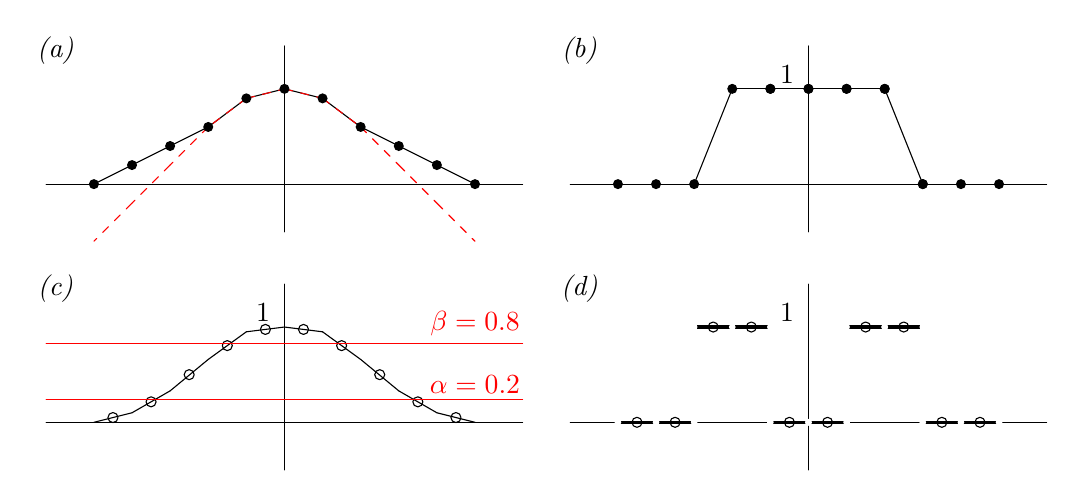
\begin{tikzpicture}[line cap=round,line join=round,>=triangle 45,scale=1.21]

%%%%%% (a) %%%%%
    \draw (0.4,0.9) -- (0.8,0.6);
    \draw (0.8,0.6) -- (1.2,0.4);
    \draw (1.2,0.4) -- (1.6,0.2);
    \draw (-0.4,0.9) -- (-0.8,0.6);
    \draw (-0.8,0.6) -- (-1.2,0.4);
    \draw (-1.2,0.4) -- (-1.6,0.2);
    \draw (-1.6,0.2) -- (-2,0);
    \draw (1.6,0.2) -- (2,0);
    \draw (-0.4,0.9) -- (0,1);
    \draw (0,1) -- (0.4,0.9);

    % New red curve aligning with black nodes
    \draw[red,dashed] (1.6,-.2) -- (2,-.6);
    \draw[red,dashed] (1.2,0.2) -- (1.6,-.2);
    \draw[red,dashed] (0.8,0.6) -- (1.2,0.2);
    \draw[red,dashed] (0.4,0.9) -- (0.8,0.6);
    \draw[red,dashed] (0,1) -- (0.4,0.9);
    \draw[red,dashed] (-0.4,0.9) -- (0,1);
    \draw[red,dashed] (-0.4,0.9) -- (-0.8,0.6);
    \draw[red,dashed] (-0.8,0.6) -- (-1.2,.2);
    \draw[red,dashed] (-1.2, .2) -- (-1.6,-.2);
    \draw[red,dashed] (-1.6,-.2) -- (-2,-.6);

    \begin{scriptsize}
      \fill [color=black] (-0.4,0.9) circle (1.5pt);
      \fill [color=black] (0.4,0.9) circle (1.5pt);
      \fill [color=black] (0.8,0.6) circle (1.5pt);
      \fill [color=black] (1.2,0.4) circle (1.5pt);
      \fill [color=black] (1.6,0.2) circle (1.5pt);
      \fill [color=black] (-0.8,0.6) circle (1.5pt);
      \fill [color=black] (-1.2,0.4) circle (1.5pt);
      \fill [color=black] (-1.6,0.2) circle (1.5pt);
      \fill [color=black] (-2,0) circle (1.5pt);
      \fill [color=black] (2,0) circle (1.5pt);
      \fill [color=black] (0,1) circle (1.5pt);
    \end{scriptsize}

    % Add Axes
    \draw[-] (-2.5,0) -- (2.5,0); % x-axis
    \draw[-] (0,-0.5) -- (0,1.45); % y-axis

    \node at (-2.4,1.4) {\emph{(a)}};


%%%%%% (b) %%%%%
\begin{scope}[shift={(5.5,0.0)}]
    \draw (1.6,0) -- (2,0);
    \draw (1.2,0) -- (1.6,0);
    \draw (0.8,1) -- (1.2,0);
    \draw (0.4,1) -- (0.8,1);
    \draw (0,1) -- (0.4,1);
    \draw (-0.4,1) -- (0,1);
    \draw (-0.4,1) -- (-0.8,1);
    \draw (-0.8,1) -- (-1.2,0);
    \draw (-1.2,0) -- (-1.6,0);
    \draw (-1.6,0) -- (-2,0);

    % Add black vertices
    \begin{scriptsize}
      \fill [color=black] (1.6,0) circle (1.5pt);
      \fill [color=black] (2,0) circle (1.5pt);
      \fill [color=black] (1.2,0) circle (1.5pt);
      \fill [color=black] (0.8,1) circle (1.5pt);
      \fill [color=black] (1.2,0) circle (1.5pt);
      \fill [color=black] (0.4,1) circle (1.5pt);
      \fill [color=black] (0.8,1) circle (1.5pt);
      \fill [color=black] (0,1) circle (1.5pt);
      \fill [color=black] (0.4,1) circle (1.5pt);
      \fill [color=black] (-0.4,1) circle (1.5pt);
      \fill [color=black] (0,1) circle (1.5pt);
      \fill [color=black] (-0.4,1) circle (1.5pt);
      \fill [color=black] (-0.8,1) circle (1.5pt);
      \fill [color=black] (-1.2,0) circle (1.5pt);
      \fill [color=black] (-1.6,0) circle (1.5pt);
      \fill [color=black] (-2,0) circle (1.5pt);
    \end{scriptsize}
    
    % Add Axes
    \draw[-] (-2.5,0) -- (2.5,0); % x-axis
    \draw[-] (0,-0.5) -- (0,1.45); % y-axis

    % Label y=1
    \node at (-0.05,1.15) [left] {1};

    \node at (-2.4,1.4) {\emph{(b)}};
\end{scope}


%%%%%% (c) %%%%%
\begin{scope}[shift={(0.0,-2.5)}]
    % Draw the smoothed curve
    \draw (1.6, 0.1) -- (2,0);      
    \draw (1.2, 0.33) -- (1.6, 0.1);
    \draw (0.8, 0.66) -- (1.2, 0.33);
    \draw (0.4, 0.95) -- (0.8, 0.66);
    \draw (0,1) -- (0.4, 0.95);
    \draw (-0.4, 0.95) -- (0,1);
    \draw (-0.4, 0.95) -- (-0.8, 0.66);
    \draw (-0.8, 0.66) -- (-1.2, 0.33);
    \draw (-1.2, 0.33) -- (-1.6, 0.1);
    \draw (-1.6, 0.1) -- (-2,0);

    % Add black circles at element centers
    \begin{scriptsize}
      \draw [color=black] (1.8, 0.05) circle (1.5pt);
      \draw [color=black] (1.4, 0.215) circle (1.5pt);
      \draw [color=black] (1.0, 0.5) circle (1.5pt);
      \draw [color=black] (0.6, 0.805) circle (1.5pt);
      \draw [color=black] (0.2, 0.975) circle (1.5pt);
      \draw [color=black] (-0.2, 0.975) circle (1.5pt);
      \draw [color=black] (-0.6, 0.805) circle (1.5pt);
      \draw [color=black] (-1.0, 0.5) circle (1.5pt);
      \draw [color=black] (-1.4, 0.215) circle (1.5pt);
      \draw [color=black] (-1.8, 0.05) circle (1.5pt);
    \end{scriptsize}

    % Add Axes
    \draw[-] (-2.5,0) -- (2.5,0); % x-axis
    \draw[-] (0,-0.5) -- (0,1.45); % y-axis

    % Label y=1
    \node at (-0.05,1.15) [left] {1};

    % Add red horizontal lines; pretend heights are 0.8 and 0.2
    \draw[red] (-2.5, 0.83) -- (2.5, 0.83);
    \draw[red] (-2.5, 0.24) -- (2.5, 0.24);
    % Label the heights of the red lines
    \node[red] at (2, 0.8) [above] {$\beta=0.8$};
    \node[red] at (2, 0.2) [above] {$\alpha=0.2$};

    \node at (-2.4,1.4) {\emph{(c)}};
\end{scope}


%%%%%% (d) %%%%%
\begin{scope}[shift={(5.5,-2.5)}]

    \draw[very thick] (1.6,0) -- (2,0);      
    \draw[very thick] (1.2,0) -- (1.6,0);
    \draw[very thick] (0.8,1) -- (1.2,1);
    \draw[very thick] (0.4,1) -- (0.8,1);
    \draw[very thick] (0,0) -- (0.4,0);
    \draw[very thick] (-0.4,0) -- (0,0);
    \draw[very thick] (-0.4,1) -- (-0.8,1);
    \draw[very thick] (-0.8,1) -- (-1.2,1);
    \draw[very thick] (-1.2,0) -- (-1.6,0);
    \draw[very thick] (-1.6,0) -- (-2,0);

    % Add Axes
    \draw[-] (-2.5,0) -- (2.5,0); % x-axis
    \draw[-] (0,-0.5) -- (0,1.45); % y-axis

    % Label y=1
    \node at (-0.05,1.15) [left] {1};

    % Add Nodes in white to separate elements
    \begin{scriptsize}
    \fill [color=white] (1.6,0) circle (1.0pt);
    \fill [color=white] (2,0) circle (1.0pt);      
    \fill [color=white] (1.2,0) circle (1.0pt);
    \fill [color=white] (0.8,1) circle (1.0pt);
    \fill [color=white] (1.2,1) circle (1.0pt);
    \fill [color=white] (0.4,1) circle (1.0pt);
    \fill [color=white] (0.8,1) circle (1.0pt);
    \fill [color=white] (0,0) circle (1.0pt);
    \fill [color=white] (0.4,0) circle (1.0pt);
    \fill [color=white] (-0.4,0) circle (1.0pt);
    \fill [color=white] (0,0) circle (1.0pt);
    \fill [color=white] (-0.4,1) circle (1.0pt);
    \fill [color=white] (-0.8,1) circle (1.0pt);
    \fill [color=white] (-1.2,1) circle (1.0pt);
    \fill [color=white] (-1.2,0) circle (1.0pt);
    \fill [color=white] (-1.6,0) circle (1.0pt);
    \fill [color=white] (-2,0) circle (1.0pt);
    \end{scriptsize}

    % Add black circles at element centers
    \begin{scriptsize}
      \draw [color=black] (1.8, 0.0) circle (1.5pt);
      \draw [color=black] (1.4, 0.0) circle (1.5pt);
      \draw [color=black] (1.0, 1.0) circle (1.5pt);
      \draw [color=black] (0.6, 1.0) circle (1.5pt);
      \draw [color=black] (0.2, 0.0) circle (1.5pt);
      \draw [color=black] (-0.2, 0.0) circle (1.5pt);
      \draw [color=black] (-0.6, 1.0) circle (1.5pt);
      \draw [color=black] (-1.0, 1.0) circle (1.5pt);
      \draw [color=black] (-1.4, 0.0) circle (1.5pt);
      \draw [color=black] (-1.8, 0.0) circle (1.5pt);
    \end{scriptsize}

    \node at (-2.4,1.4) {\emph{(d)}};
\end{scope}

\end{tikzpicture}
  
\caption{Illustration of VCD: \emph{(a)} The function $u_h$ (solid) is an approximate solution to \eqref{eq:fe:vi}, with nodes $x_j$ shown (solid dots), and obstacle $\psi_h$ (red dashed).  \emph{(b)} Nodal active set indicator $\nu_h \in \CG_1(\cT_h)$, with values in $\{0,1\}$.  \emph{(c)} Smoothed indicator $s_h$ (solid), with element degrees of freedom $x_k$ (circles) and thresholding levels shown (red).  \emph{(d)} Element marking $I_h$; 4 elements are marked for refinement.}
\label{fig:vcdillustration}
\end{figure}

The third AMR method in this section is based on \emph{metric-based mesh adaptation} \cite{Alauzet2010}.  Instead of marking elements for refinement, such mesh adaptation effectively both refines and coarsens to match mesh complexity and resolution target values, for example to keep the mesh complexity approximately constant.  Adaptation is driven by an \emph{a posteriori} computed \emph{metric (field)}, which is a continuous, matrix-valued function $M_h:\Omega \to \RR^{d\times d}$.  Each point value $M_h(x)$ is a symmetric and positive-definite matrix.  Such a metric contains local information on distances, areas, and volumes, analogous to a continuous version of a mesh; the analogy can be made precise \cite{LoseilleAlauzet2011}.  The construction of the metric field depends on the meshing goal.  The mesher itself generates a unit mesh with respect to the given metric field, which becomes a mesh with anisotropic edge lengths in the original space \cite{Wallworketal2020}.

Our \emph{averaged-metric} (AVM) AMR method for VIs starts from $u_h$ and $\psi_h$.  The first metric $M_1(x)$ is computed from the gradient of a smoothed nodal active set indicator, namely $s_h$ from the VCD method (Algorithm \ref{alg:vcd}) above.  The metric is isotropic because it is a multiple of the identity: $M_1(x) = c_1 |\grad s_h(x)| I_{d\times d}$.  The second metric $M_2(x)$ is an approximate Hessian of $u_h$, computed via a Hessian-recovery technique \cite{Alauzet2010} because the FE function $u_h$ generally has discontinuous first derivatives.  Actually the absolute value of the Hessian, well-defined because the Hessian is a symmetric matrix \cite{Wallworketal2020}, is used to produce an anisotropic metric: $M_2(x) = c_2 |H u_h(x)|$.  These metrics are computed in the matrix-valued $\CG_1$ FE space, and $c_1,c_2$ are metric normalization constants computed in a standard manner \cite{Wallworketal2020}.  By construction, the first metric should generate small elements near the free boundary, while the second metric should reduce FE approximation error, specifically in the inactive set, because the Hessian of the continuous solution $u$ appears in standard interpolation theory \cite{Wallworketal2020}.

The final metric seen by the mesher is then a weighted average:
\begin{equation} \label{eq:avm}
M_h(x) = \gamma M_1(x) + (1-\gamma) M_2(x) = \gamma c_1 |\grad s_h(x)| I_{d\times d} + (1-\gamma) c_2 |H u_h(x)|,
\end{equation}
where $\gamma \in [0,1]$; the default is $\gamma=0.5$.  This result $M_h(x)$ is an anisotropic metric which is free-boundary aware.  Our implementation of the AVM method calls the Animate library (\href{https://github.com/mesh-adaptation/animate}{{\small \texttt{github.com/mesh-adaptation/animate}}}) to construct the metrics $M_i(x)$, and to compute their average $M_h$.  Note that Animate uses the Pragmatic library (\href{https://github.com/meshadaptation/pragmatic}{{\small \texttt{github.com/meshadaptation/pragmatic}}}) as the default metric-based mesher.

Recall that Figure \ref{fig:threeballmeshes} shows AMR results from all three methods on the ``ball'' obstacle problem shown in Figures \ref{fig:ball} and \ref{fig:activesizes} (middle).  The right sub-figure shows an AVM result for this problem.  Note that iterating the AVM method, even while holding the target mesh complexity constant, is worthwhile because the increased resolution near the free boundary allows the \emph{a posteriori}-determined metric to become more effective.  However, because of the many nontrivial computations in metric-based methods \cite{Alauzet2010,Wallworketal2020}, one iteration of AVM is substantially more expensive than an iteration of UDO, even when adding a residual-based marking in the inactive set like \eqref{eq:brestimator}; see Section \ref{sec:results}.

All three methods, UDO, VCD, and AVM, run in parallel under the MPI process model used by Firedrake/PETSc \cite{Bueler2021,Langeetal2016}.  However, only UDO produces identical results independent of the number of processes.  The VCD method can be configured to have this property, namely by choosing a direct solver for problem \eqref{eq:diffusioneqn}, but this reduces scalability.  For VCD the use of the preconditioned Krylov solver is preferred, though its default parallel block preconditioner will generate slightly different results depending on number of processes \cite{Bueler2021}.

We end this section with two basic Python examples which show how the library, available open source at \href{https://github.com/StefanoFochesatto/VI-AMR}{{\small \texttt{github.com/StefanoFochesatto/VI-AMR}}}, is used.

\begin{example} \label{example:AOL}
Consider Example 1 from \cite{AinsworthOdenLee1993}, a classical obstacle problem over a rectangle, with obstacle $\psi=0$ and a known exact solution.  The complete code below, which applies the Firedrake and VIAMR libraries, generates a coarse mesh and then applies VCD marking and refinement around the free boundary.  The initial mesh, marked elements near the free boundary, and refined mesh are shown in Figure \ref{fig:resultAOL}.
\inputminted[linenos, frame=lines]{python}{../examples/aol.py}
\end{example}

\begin{figure}[ht]
\centering
\mbox{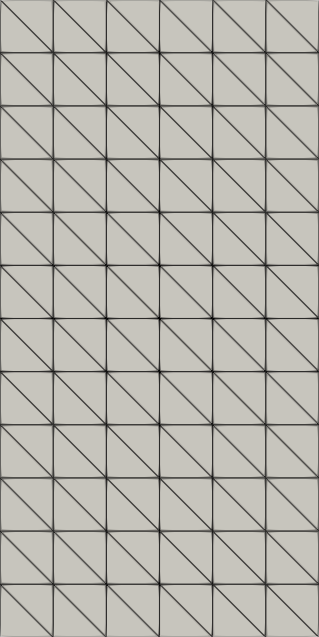
\includegraphics[width=0.21\textwidth]{static/aol-mesh0.png} \qquad\quad
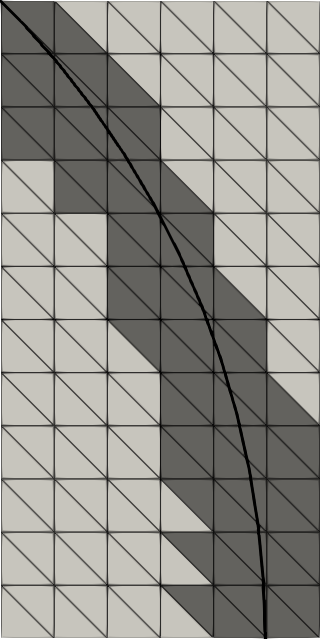
\includegraphics[width=0.21\textwidth]{static/aol-marked.png} \qquad\quad
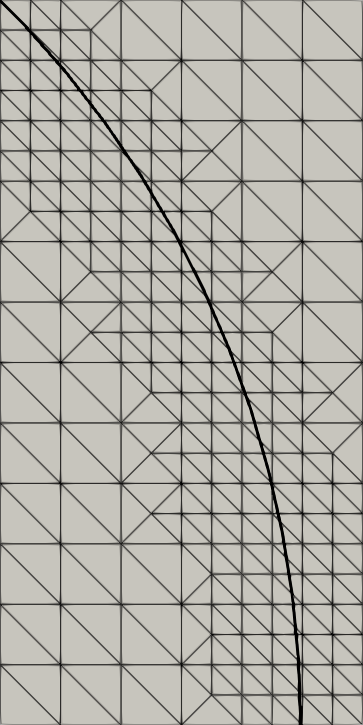
\includegraphics[width=0.21\textwidth]{static/aol-mesh1.png}}
\caption{The Python code in Example \ref{example:AOL}, which solves Example 1 from \cite{AinsworthOdenLee1993}, starts from an initial mesh (left), marks elements by the default-parameter VCD scheme (middle), and generates a refined mesh (right).  The exact free boundary, unknown to the algorithm, is overlaid in black.}
\label{fig:resultAOL}
\end{figure}

\begin{example} \label{example:hybrid}
For the left-hand mesh in Figure \ref{fig:threeballmeshes}, after computing the FE solution \texttt{uh} on each mesh level, the following code snippet generate the next refined mesh:
\begin{minted}[linenos, frame=lines]{python}
amr = VIAMR()
residual = -div(grad(uh))
imark, _, _ = amr.brinactivemark(uh, psi, residual, theta=0.7)
fbmark = amr.udomark(uh, psi, n=1)
mark = amr.unionmarks(fbmark, imark)
mesh = amr.refinemarkedelements(mesh, mark)
\end{minted}
Here the BR error indicator (Section \ref{sec:aposteriori}) for the inactive set is computed from the \emph{a posteriori} element-wise residual, and then the $n=1$ case of UDO is used to mark near the free boundary, and finally these marks are unioned (hybridized).
\end{example}



\section{Results} \label{sec:results}

FIXME discuss norm and geometric measures first

FIXME \cite{Kosub2016} \cite{JungeblutKleistMiltzow2022}

FIXME


\section{Application to determining glaciated areas} \label{sec:app}

In this section we apply AMR techniques to a model for steady glacier geometry over a given bedrock topography and with a given climate.  A goal of this model is to determine the land which is covered by glaciers, and to determine the ice volume.  Though a glacier covers any land on which snowfall dominates melt, ice flow further expands the glacier out to a free boundary.  This glacier margin can only be determined by solving the coupled mass and momentum equations.

Here the unknown thickness is constrained to be nonnegative, the operator is nonlinear, and the VI problem is \emph{not} of optimization type (for general bedrock).  Similar problems arise for any fluid layer subject to surface processes which add or remove mass \cite{Bueler2021b}.  They have the ``blistering'' property mentioned in the Introduction (and \cite{JouvetBueler2012}).

Let $\Omega \subset \RR^2$ be a fixed land region, and choose a bedrock elevation $b \in C^1(\Omega)$.  Let $a \in L^2(\Omega)$ be a surface mass-balance function \cite{GreveBlatter2009}, the annually-averaged rate of ice accumulation (snow) minus melt and runoff, which is the ``climate'' experienced by the glacier.  (Here distances and elevations are in meters, and $a$ is in meters per second.)  We consider a glacier flow approximation called the \emph{shallow ice approximation} \cite{GreveBlatter2009}, in the simple isothermal and non-sliding case.   For the standard exponent for the flow law of ice \cite{GreveBlatter2009} we have a VI for the transformed ice thickness $u\in \cX = W^{1,4}(\Omega)$ such that $u\ge 0$; the thickness itself is $H=u^{3/8}$.  Let $\cK = \{u \in \cX\,:\,u\ge 0 \text{ and } u|_{\partial\Omega}=0\}$.  The model uses a ``tilted'' $p$-Laplacian operator \cite{JouvetBueler2012}; we seek $u\in\cK$ so that
\begin{equation}
\int_\Omega \Gamma |\grad u + \bm{\beta}(u)|^2 (\grad u + \bm{\beta}(u)) \cdot \grad (v-u) \,dx \ge \int_\Omega a (v-u)\,dx \quad \text{ for all } v \in \cK. \label{eq:siavi}
\end{equation}
Here $\Gamma>0$ is a physical constant, essentially the ice softness, and $\bm{\beta}(u)=\frac{8}{3} u^{5/8} \grad b$ is a nonlinear multiple of the bed gradient.  The left side of \eqref{eq:siavi} defines a nonlinear operator $F(u)[v-u]$ which is $4$-coercive (definition \eqref{eq:coercive}) if $\grad b=0$.

While uniqueness for \eqref{eq:siavi} is generally open, existence always holds \cite{JouvetBueler2012}, and when $\grad b=0$ the problem is well-posed.  Note that the thickness $H$ and the conserved flux $\bq = - \Gamma |\grad u + \bm{\beta}(u)|^2 (\grad u + \bm{\beta}(u))$ go to zero at the margin.  However, observations of glaciers confirm that the gradient of the surface has large magnitude as one approaches the margin from the icy side, a property which emerges from a solution to \eqref{eq:siavi} when one computes the associated surface elevation $s=H+b = u^{3/8} + b$.

For this highly-nonlinear problem we apply FE with $u_h\in\CG_1(\cT_h)$.  The problem is solved either by the same VI-adapted Newton solver as in Section \ref{sec:results}, or adding an outer Picard-type iteration over the tilt $\bm{\beta}(u)$ \cite{JouvetBueler2012}, with similar results; the latter solver is more robust when $|\grad b|$ is large.  We consider two particular problems over a square domain $\Omega=(0,L)^2$, $L=1800$ kilometers: \emph{i)} ``dome'' problem with a flat bed and known solution \cite{Bueler2016} and \emph{ii)} ``cap'' problem with a bumpy bed \cite[Example 8.4]{BuelerFarrell2024}.

Our goals are to generate meshes with high resolution along an accurately-estimated glacier margin.  The UDO and VCD tag-and-refine methods are compared, with a gradient-recovery (GR) error indicator in the inactive set.  (See Example \ref{example:gradrecovery}; note that the linear derivation of the BR error indicator in Example \ref{example:br} does not apply.)  Figure \ref{fig:glacier} shows sample results for the cap problem, including the mesh after three levels of AMR starting from a coarse, uniform mesh (left), and a detail of the jump in the surface gradient at a highly-refined margin with element size around $h = 100$ meters (right).

% $ cd examples/glacier
%LEFT:
% $ python3 steady.py -prob cap -newton -m 7 -opvd result_cap.pvd
% $ paraview result_cap.pvd
%RIGHT:
% $ tmpg -n 12 python3 steady.py -newton -m 5 -refine 11 -prob cap -opvd result_cap_11.pvd
% $ paraview result_cap_11.pvd
\begin{figure}[ht]
\centering
\mbox{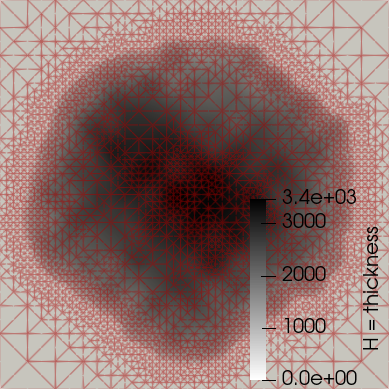
\includegraphics[width=0.46\textwidth]{static/glacier/thickness.png} \qquad 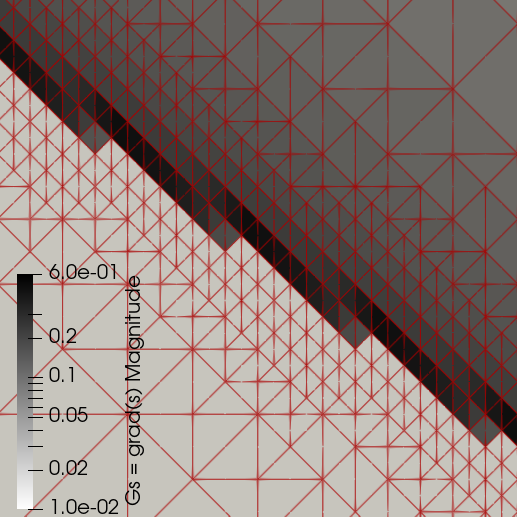
\includegraphics[width=0.46\textwidth]{static/glacier/detail.png}}
\caption{Left:  Ice thickness (grayscale; meters) with a mesh (red) found by applying UDO and a gradient-recovery indicator in the inactive set.  Right:  A detail of the glacier margin at higher refinement.  Though $|\grad u|$ is continuous, the surface elevation gradient $|\grad s|$ (grayscale magnitude) is discontinuous at the margin.}
\label{fig:glacier}
\end{figure}

% FIXME consider showing $\|H-H_h\|_{L^\infty}$ in meters instead of relative

The dome problem was solved with 13 levels of refinement from an initial, uniform $h_0=360$ kilometer mesh to a final mesh with margin resolution of $h_{13}\approx 30$ meters.  Figure \ref{fig:domenormresults} shows $\cX=H^1$ errors in the solution ($\|u-u_h\|_{H^1}/\|u\|_{H^1}$) and $L^\infty$ errors in the corresponding ice thickness ($\|H-H_h\|_{L^\infty}/\|H\|_{L^\infty}$), versus number of elements.  Note that in these runs solver time was observed to closely track number of elements, so showing run-times would add no information.

% UNIFORM:  tmpg -n 12 python3 steady.py -newton -m 5 -refine 8 -uniform 8 -csv uniform.csv
% UDO+GR:   tmpg -n 12 python3 steady.py -newton -m 5 -refine 13 -csv udo.csv
% VCD+GR:   tmpg -n 12 python3 steady.py -newton -m 5 -refine 13 -vcd -csv vcd.csv
\begin{figure}[ht]
\noindent\mbox{\includegraphics[width=0.49\textwidth]{genfigs/uerrh1.png} \, \includegraphics[width=0.49\textwidth]{genfigs/herrinf.png}}
\caption{Left: Per element, $H^1$ norm errors in $u$ are comparable for AMR methods and uniform refinement.  Right: Because of low regularity at the ice margin, maximum ice thickness error is large, but AMR is effective in reducing it.}
\label{fig:domenormresults}
\end{figure}

Figure \ref{fig:domeradiusresults} addresses free-boundary localization.  We compute the maximum distance between free-boundary nodes and the exact, circular margin, which reveals that the AMR methods locate the free boundary much more efficiently than uniform refinement.  Given the large ice thickness gradients at the free boundary, this also explains why $\|H\|_{L^\infty}$ errors are more responsive to AMR than $\|u\|_{H^1}$ errors (Figure \ref{fig:domenormresults}).

\begin{figure}[ht]
\centering
\includegraphics[width=0.51\textwidth]{genfigs/drmax.png}
\caption{AMR generates accurate free boundary locations.  At $10^7$ elements the glacier margin is located within tens of meters, versus a kilometer for uniform refinement.}
\label{fig:domeradiusresults}
\end{figure}


\section{Discussion and conclusion} \label{sec:conclusion}

FIXME \emph{Grid Sequencing + AMR targeting the free boundary} is the iterative process for how we are converging to the FB.  The bulk of vinewton iterations are coming from stabilizing the initial iterate's FB and thereafter Grid Sequencing is allowing us to make small adjustments as we refine.  the grid sequencing works best on hierarchal meshes, while with metric method the "grid sequencing" is done through cross-mesh interpolation.

FIXME We have no quantitative theory (norm bounds) telling us how the two strategies interact.  We are applying two different, well-defined, marking strategies:
\begin{enumerate}
\item assuming $u_h$ gives an estimate of the free boundary, mark nearby elements on both sides of the free boundary
\item assuming $u_h$ gives an estimate of the inactive set, mark in this approximate inactive set according to PDE principles
\end{enumerate}
Note that i) has nothing directly to do with the regularity (or residual) in $u_h$.  Regardless of the smoothness of $u_h$ near the free boundary, or the magnitude of the residual from $u_h$, we want to mark near the free boundary.

FIXME integration with multilevel strategy in \cite{BuelerFarrell2024} is TODO

%\section*{Acknowledgements}

%\section*{Notes on contributor(s)}
%An unnumbered Section, e.g.\ \verb"\section*{Notes on contributors}", may be included \emph{in the non-anonymous version} if required. A photograph may be added if requested.


\section{References}

\bibliographystyle{tfs}
\bibliography{viamr}


%Any appendices should be placed after the list of references, beginning with the command \verb"\appendix" followed by the command \verb"\section" for each appendix title, e.g.
%\appendix
%\section{This is the title of the first appendix}

\end{document}
